%%%%%%%%%%%%%%%%%%%%%%%%%%%%%%%%%%%%%%%%%%%%%%%%%%%%%%%%%%%%%%%%%%%%%%%%%%%

\documentclass{standalone}

\usepackage{amsmath}
\usepackage{mathptmx}
\usepackage{pgfplots}
\usetikzlibrary{external}
\tikzexternalize{sunshine-vary-c}
\pgfplotsset{compat=1.16}

%% IEEE uses Times Roman font, so we'll default to Times.
%% These three commands make up the entire times.sty package.
\renewcommand{\rmdefault}{ptm}
\renewcommand{\ttdefault}{pcr}
\normalfont\selectfont

\begin{document}

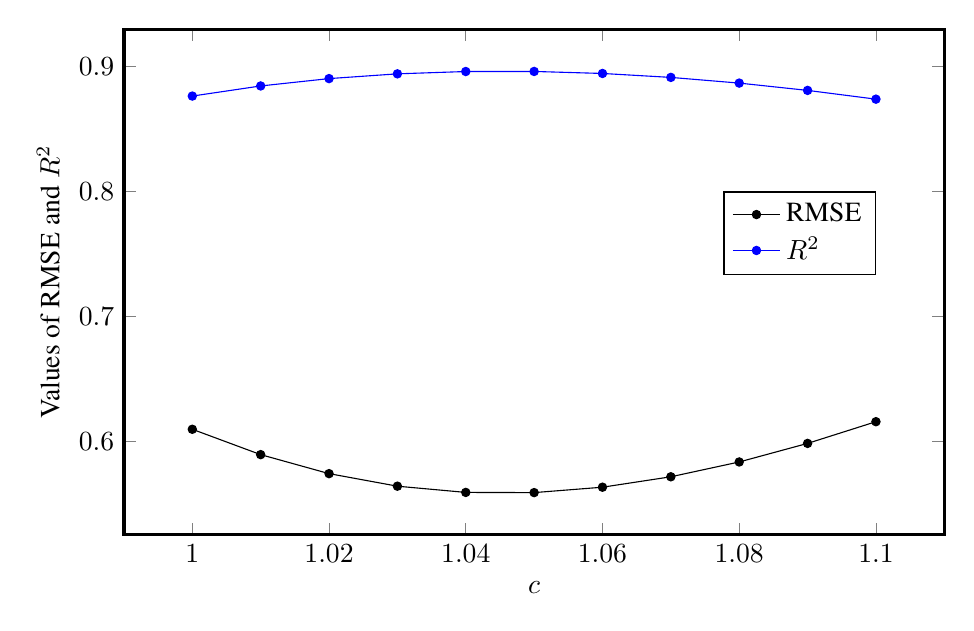
\begin{tikzpicture}
\tikzset{%%
  every mark/.append style={scale=1.0},%%
  scale=1.0%%
}
\pgfplotsset{%%
  every axis/.append style={font=\normalsize}%%
}
%%
\begin{axis}[%%
  axis line style=very thick,%%
  dotStyle/.style={mark size=1.5,mark color=black,mark=*},%%
  enlargelimits=true,%%
  height=8cm,%%
  legend cell align=left,%%
  legend style={at={(axis cs:1.1,0.8)},anchor=north east},%%
  width=12cm,%%
  %% x axis
  xlabel={\normalsize $c$},%%
  %% y axis
  ylabel={\normalsize Values of RMSE and $R^2$}%%
]
%%
%%
%% The change in the values of the RMSE.
\addplot[dotStyle,black] coordinates {
  (1.00, 0.609530)
  (1.01, 0.589218)
  (1.02, 0.574005)
  (1.03, 0.563949)
  (1.04, 0.558963)
  (1.05, 0.558812)
  (1.06, 0.563137)
  (1.07, 0.571484)
  (1.08, 0.583350)
  (1.09, 0.598218)
  (1.10, 0.615595)
};
\addlegendentry{RMSE}
%%
%%
%% The change in the values of R^2.
\addplot[dotStyle,blue] coordinates {
  (1.00, 0.876352)
  (1.01, 0.884456)
  (1.02, 0.890345)
  (1.03, 0.894154)
  (1.04, 0.896017)
  (1.05, 0.896073)
  (1.06, 0.894458)
  (1.07, 0.891306)
  (1.08, 0.886746)
  (1.09, 0.880899)
  (1.10, 0.873879)
};
\addlegendentry{$R^2$}
\end{axis}
\end{tikzpicture}

\end{document}
